\documentclass[11pt]{article}
\usepackage{geometry}                % See geometry.pdf to learn the layout options. There are lots.
\geometry{letterpaper}                   % ... or a4paper or a5paper or ... 
%\geometry{landscape}                % Activate for for rotated page geometry
%\usepackage[parfill]{parskip}    % Activate to begin paragraphs with an empty line rather than an indent
\usepackage{graphicx}
\usepackage[colorinlistoftodos]{todonotes}
\usepackage{amssymb}
\usepackage{epstopdf}
\usepackage[english]{babel}
\usepackage{placeins}
\usepackage{tikz}
\usepackage{pgf}
\usepackage{inputenc}
\usetikzlibrary{shapes,arrows}
\usetikzlibrary{automata,positioning}     
\usepackage{listings}
\usepackage{smartdiagram}
\usepackage{tocstyle}
\usetocstyle{standard}
\lstset
{ %Formatting for code in appendix
    language = C,
    basicstyle=\footnotesize,
}   

\tikzset{
    state/.style={
           rectangle,
           rounded corners,
           draw=black, very thick,
           minimum height=2em,
           inner sep=2pt,
           text centered,
           },
}
\DeclareGraphicsRule{.tif}{png}{.png}{`convert #1 `dirname #1`/`basename #1 .tif`.png}
\begin{document}
\begin{titlepage}

\newcommand{\HRule}{\rule{\linewidth}{0.5mm}} % Defines a new command for the horizontal lines, change thickness here

\center % Center everything on the page
 
%----------------------------------------------------------------------------------------
%	HEADING SECTIONS
%----------------------------------------------------------------------------------------

\textsc{\LARGE George Mason University}\\[1.5cm] % Name of your university/college


%----------------------------------------------------------------------------------------
%	TITLE SECTION
%----------------------------------------------------------------------------------------

\HRule \\[0.4cm]
{ \huge \bfseries Implementing OTA Updates for an IoT Security Device}\\[0.4cm] % Title of your document
\HRule \\[1.5cm]
 
%----------------------------------------------------------------------------------------
%	AUTHOR SECTION
%----------------------------------------------------------------------------------------
\begin{minipage}{0.4\textwidth}
\begin{flushleft} \large
\emph{Authors:}\\
Gerson \textsc{Dalton Cardozo} \\
M. Sohail \textsc{Iqbal} \\ 
Aneesh \textsc{Malhotra} \\ 
Mohamed \textsc{Nur} \\ 
Ryan \textsc{Thomas} % Your name 
\end{flushleft}
\end{minipage}
~
\begin{minipage}{0.4\textwidth}
\begin{flushright} \large
\emph{Supervisor:} \\
Dr. Jens-Peter \textsc{Kaps} % Supervisor's Name
\end{flushright}
\end{minipage}\\[2cm]

% If you don't want a supervisor, uncomment the two lines below and remove the section above
%\Large \emph{Author:}\\
%John \textsc{Smith}\\[3cm] % Your name

%----------------------------------------------------------------------------------------
%	DATE SECTION
%----------------------------------------------------------------------------------------

{\large \today}\\[2cm] % Date, change the \today to a set date if you want to be precise

%----------------------------------------------------------------------------------------
%	LOGO SECTION
%----------------------------------------------------------------------------------------


\includegraphics{watermark2.jpg}\\[1cm] % Include a department/university logo - this will require the graphicx package
 
%----------------------------------------------------------------------------------------

\vfill % Fill the rest of the page with whitespace

\end{titlepage}
\clearpage
\tableofcontents
\clearpage
\section{Executive Summary}

This project will build upon a previous ECE 492 project \textit{FPGA Enhanced Wireless Sensor Node for IoT Applications}. The project sought to use an FPGA to enhance the security of a wireless sensor node network while maintaining low power consumption. The network that this was implemented on was an in-home security system, which detects motion using an IR sensor on a node, and sends a picture of the intruder to the user via the gateway. Security can be an issue in wireless sensor networks and it may be necessary to update the private key of compromised node or update the firmware of a node to enhance its performance and functionality. The most efficient and inexpensive way to distribute such an update to many users without having to dismantle the system is over-the-air (OTA). In this process a manufacturer will distribute a secure update to its users and the system will update its own firmware. Our goal in this project is to provide OTA update capability to the in-home security system developed by the previous group. 
\clearpage
\section{Approach}
\subsection{Motivation}

Many IoT devices now use wireless-sensor networks in which a user is able to control several devices called "nodes" through a single device called a "gateway". These kinds of networks are used in many popular smart home devices such as Google's Nest and Phillips Hue, most of which already provide OTA update capability. Additionally, security for these networks is becoming a concern. Wireless sensor networks are often deployed to monitor and respond to events occurring in the environment and are meant to be left unattended, making them susceptible to a variety of attacks \cite{sen_security_2013}. With the versatile capabilities of FPGA's, we see many researchers using FPGA's to enhance the capabilities of wireless sensor networks, including security \cite{g_elliptic_2016}. As FPGA's make their way into more wireless sensor networks, we will need to be able to be able to equip them with OTA update capability. Our goal is to provide this capability to our network that uses an FPGA for enhanced security. 


\subsection{Problem Analysis}
The problem we face is to be able to provide OTA updates to the node of the previous system (Figure 1). Since the node is not directly connected to a computer, we must be able to reprogram the node using only the existing hardware on the node. Additionally, the node consists of an MSP432 microcontroller and an Actel IGLOO FPGA. Updating the security features such as the private key and the algorithm on the FPGA will require us to be able to reprogram the FPGA remotely. Likewise, updating the firmware and capabilities of the microcontroller will require us to be able to reprogram the MSP432 remotely. 

\begin{figure}[!ht]
\centering
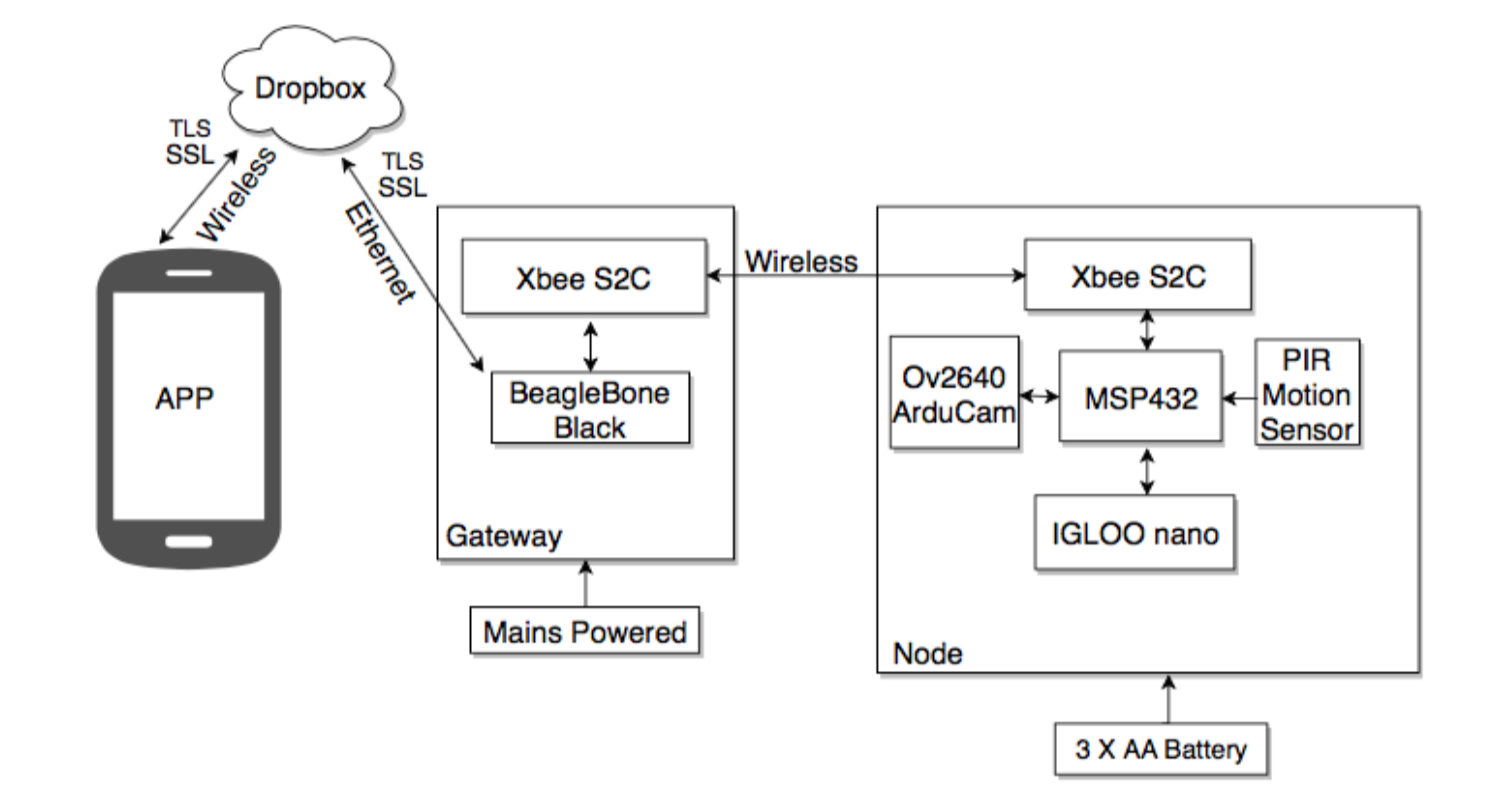
\includegraphics[scale = 0.35]{schematic1.png}
\caption{Top Level Diagram of Camera Security System}
\end{figure}
\FloatBarrier


\subsection{Solution}
Our solution to this problem is to redesign the system to be able to request updates from an external sever, download the update to the Gateway, push the update to the MSP432 via the XBee, and allow the MSP432 to reprogram both itself and the FPGA through a bootloader. The update will simply consist of a .zip file that consists of a YAML file, the updated code, and some header information. Our goal is to be able to parse the update on the Gateway, and send bootloader commands to the node. The MSP432 on the node will then use these commands to reprogram its own program memory, as well as interface to and reprogram the FGPA. 


\subsection{Components}

\begin{enumerate}
\item External Server
\begin{itemize}
\item Contains secure signature and contains update files.
\item Stores user data collected from the node such as images. 
\end{itemize}

\item Update
\begin{itemize}
\item Contains a .zip file with a YAML file as well as the source code.
\item The YAML file will have have an MSP432 and FPGA section, and will be converted to bootloader commands. 
\end{itemize}

\item Phone
\begin{itemize}
\item Provides interface to user
\item Checks for and initiates updates
\item Allows for rekeying and initiating capture from the node camera.
\end{itemize}

\item Gateway
\begin{itemize}
\item Main system component
\item Contains a BeagleBone Black running Linux and an XBee to communicate with the node
\item Parses YAML file, and maps it to bootloader commands for the MSP432. 
\item Takes in data from the node and makes it accessible to the user. 
\end{itemize}

\item Node
\begin{itemize}
\item Secondary system component
\item Contains an MSP432, Actel IGLOO FPGA, an XBee, an ArduCam v5 5MP camera, and an IR sensor. 
\item The MSP432 controls all other components and will have the capability to reprogram itself and the FPGA.
\item The node will capture an image and send it back to the Gateway. 
\end{itemize}

\end{enumerate}

\subsection{Top-Level Design} 
\begin{figure}[!ht]
\centering
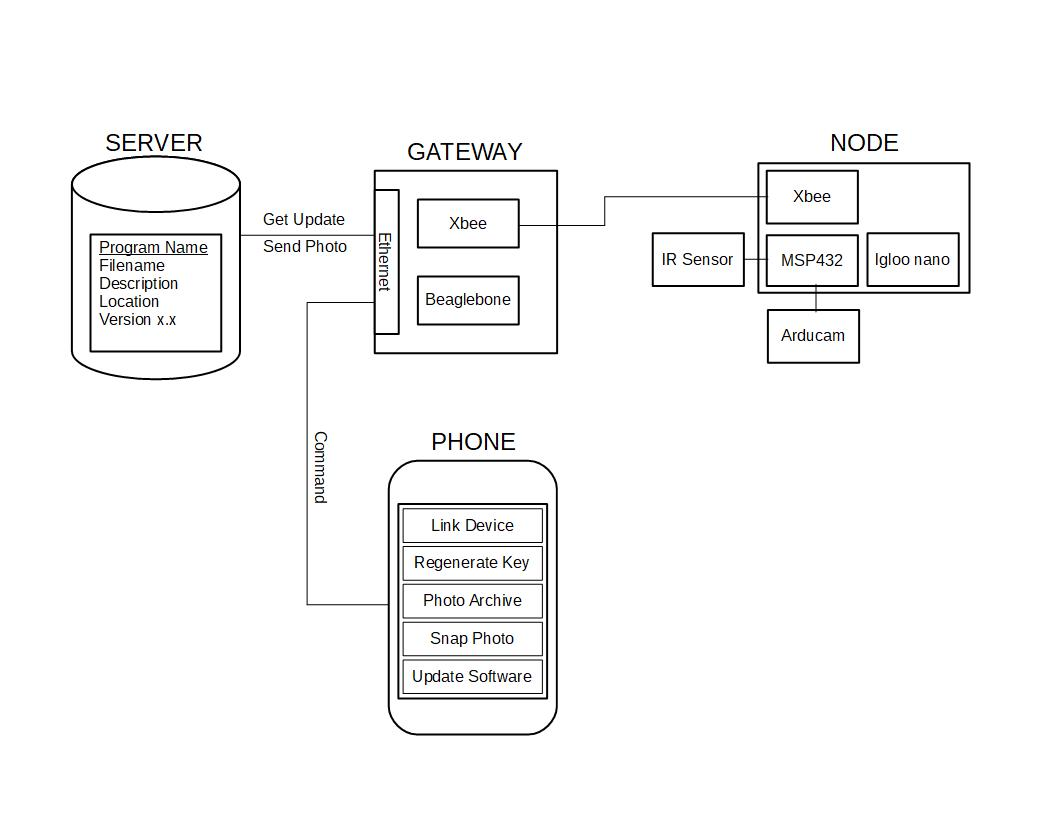
\includegraphics[scale = 0.4]{BlockDiagram.jpg}
\caption{The camera security system no longer uses Dropbox, but rather a server to host the updates.}
\end{figure}
\FloatBarrier


\begin{enumerate}
\item The server contains a file with the version number and location of an update. 
\item The user compares the version number of the update to that of the system.
\item If the version numbers do not agree, the user will have the option to begin an update. 
\item The Gateway will request the complete update, process it, push the the update and appropriate MSP432 commands to the node.
\item MSP432 will receive the update from the Gateway as well as instructions for reprogramming itself and the FPGA. This will be done via Bootloader commands. 
\end{enumerate}
\FloatBarrier

The following diagram depicts this workflow. \vspace{2em}
\begin{figure}[!ht]
\centering
\smartdiagram[flow diagram:horizontal]{Update is available,User Accepts Update ,
  Gateway Requests Update, Gateway Processing, XBee Link, MSP432 Bootloader}
  \caption{Update Workflow}
 \end{figure}


\FloatBarrier


\subsection{Alternative Designs}

\subsubsection{Dropbox}
We had initially decided to use Dropbox as a cloud storage system. Since the gateway is not a member of the local area network, this would have made communication between the Android device and the gateway to be much simpler. This communication, however, is much slower. Additionally a company pushing a firmware update to a user will not typically have access to a user's Dropbox account. A user can also accidentally delete important configuration files such as the ones used for rekeying, making it less reliable and less realistic than a dedicated server. For these reasons, we decided to use a dedicated web server for distributing updates and storing data. 


\section{System Architecture}

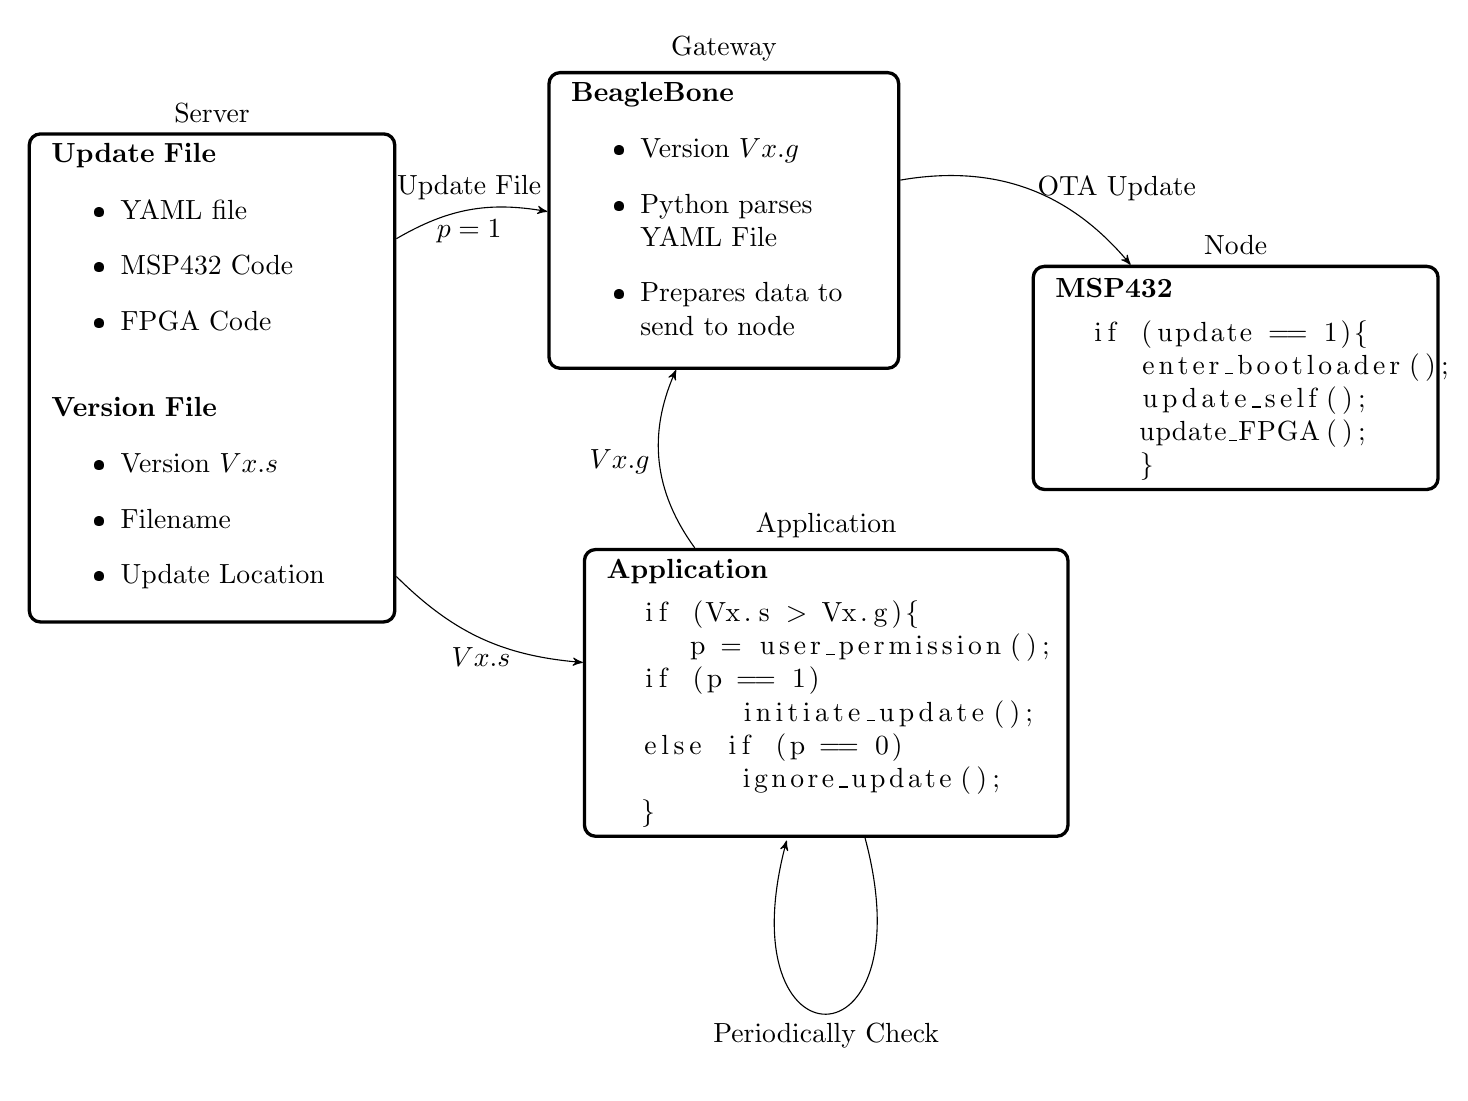
\begin{tikzpicture}[->,>=stealth']

 % Position of QUERY 
 % Use previously defined 'state' as layout (see above)
 % use tabular for content to get columns/rows
 % parbox to limit width of the listing
 \node[state, text width = 4.5cm] [label=Server](SERVER) 
 {\begin{tabular}{l}
  \textbf{Update File}\\
  \parbox{4cm}{\begin{itemize}
   \item YAML file
   \item MSP432 Code
   \item FPGA Code
  \end{itemize}
  }\\[4em]
  \textbf{Version File}\\
  \parbox{5cm}{\begin{itemize}
   \item Version $Vx.s$
   \item Filename
   \item Update Location
  \end{itemize}
  }
 \end{tabular}};
  
 % State: ACK with different content
 
 
 
 \node[state,    	% layout (defined above)
  text width=3cm, 	% max text width
  yshift=2cm, 		% move 2cm in y
  right of=SERVER, 	% Position is to the right of QUERY
  node distance=6.5cm, 	% distance to QUERY
  anchor=center,
  text width = 4.3cm][label = Gateway] (GATEWAY) 	% posistion relative to the center of the 'box'
 {%
 \begin{tabular}{l} 	% content
  \textbf{BeagleBone}\\
  \parbox{4cm}{
  \begin{itemize}
  \item Version $Vx.g$
  \item Python parses YAML File
  \item Prepares data to send to node
  \end{itemize}
  }
 
  
 \end{tabular}
 };
 
 % STATE APPLICATION
 \node[state,
  below of=GATEWAY,
  yshift=-5cm,
  xshift = 1.3cm,
  anchor=center,
  text width=6cm] [label = Application](APPLICATION) 
 {%
 \begin{tabular}{l}
  \textbf{Application}\\

  \begin{lstlisting}
  if (Vx.s > Vx.g){
     p = user_permission();
  if (p == 1)
  	initiate_update();
  else if (p == 0)
  	ignore_update();
  }
  
  \end{lstlisting}

 \end{tabular}
 };

 % STATE EPC
 \node[state,
  right of=GATEWAY,
  node distance=7cm,
  anchor=center, text width = 5cm, yshift = -2cm,xshift = -.5cm] [label = Node](NODE) 
 {%

 \begin{tabular}{l}
  \textbf{MSP432}\\

  \begin{lstlisting}
  if (update == 1){
     enter_bootloader();
     update_self(); 
     update_FPGA();
     }
  \end{lstlisting}


 \end{tabular}
 };

 % draw the paths and and print some Text below/above the graph
 \path (SERVER) 	edge[bend left=20]  node[anchor=south,above]{Update File}
                                    node[anchor=north,below]{$p = 1$} (GATEWAY)
 (SERVER)     	edge[bend right=20] node[anchor=south,below]{$Vx.s$} (APPLICATION)
 (GATEWAY)       	edge  [bend left]                      node[anchor=north,right]{OTA Update}(NODE)
 (APPLICATION)  	edge[loop below]    node[anchor=north,below]{Periodically Check} (APPLICATION)
 (APPLICATION)  	edge[bend left]         node[anchor = left, left]{$Vx.g$} (GATEWAY);

\end{tikzpicture}


\subsection{Method for MSP432}
The MSP432 can be given a \textit{bootloader}, which is a program that allows a user to access memory. By using a bootloader, we can program particular blocks of MSP432 memory corresponding to the update. These bootloaders are often available online, and have the ability to access external devices via $I^2C$, and therefore obtain incoming update information from the XBee device. 
\subsection{Method for FPGA}

Our system design architecture (shown above) shows each component involved in performing an update. Specifically, the process by which we update the FPGA using the MSP432 will be through a Jam Standard Test and Programming Language (Jam STAPL) player. This software will make it easier to send a binary bitstream to program the FGPA via the JTAG interface. We will, however, need to create an API that interfaces to the STAPL player and provides high level functions to use. The programming using this can be done both via the main function of the MSP432 and the bootloader, and we will need to decide which method to use.


\subsection{YAML File}

YAML is a data serialization language, and is essentially a tool to convert update data, which will consist of memory locations of the processor that need to be modified, and translate it into commands, specifically bootloader commands, which can be transmitted to the MSP432 through the XBee. This file will be processed on the BeagleBone Black on the Gateway using Python. 


\section{Preliminary Experimental Plan}

\begin{enumerate}
\item Our first experiment will be to see if we can successfully use the JTAG interface on the MSP432 to program the FGPA. This is a preliminary experiment to test our conceptual design and determine any further complications.
\item Our second experiment will be to simply map some bootloader commands into a YAML file, and then send them to the node. If these two tests are successful, it will verify our conceptual design and we will be able to successfully implement an update. 
\item Once the system is running completely, one goal we have is to be able to update the private key of the FPGA. We will create some code that will update the private key of the node and push that as an update to the user. 
\end{enumerate}

\section{Preliminary Project Plan}
\subsection{Tasks} 
\begin{enumerate}
\item Create an "update" to send to the system
\item Download MSP432 bootloader and learn how to interface to it
\item Download STAPL player and develop an API 
\item Construct a YAML file and write code to parse the file. 
\item Update the application to allow for an update feature.
\end{enumerate}

\subsection{Allocation of Responsibilities} 

\subsubsection{Aneesh}
\begin{itemize}
\item Project manager responsibilities such as keeping everyone on schedule.
\item Create update file, and update verification
\item Work with YAML 
\end{itemize}
\subsubsection{Ryan}
\begin{itemize}
\item Mainly responsible for writing MSP432 code to be able to reprogram itself
\end{itemize}

\subsubsection{Gerson}
\begin{itemize}
\item Create PCB design of final system, for both the gateway and the Node. 
\item Handle any issues interfacing via ZigBee to any of the devices
\end{itemize}
\subsubsection{Mohamed}
\begin{itemize}
\item Working on the application, which will interface to the server, to communicate with the gateway. 
\item Helping write code to update the BeagleBone on the Gateway
\end{itemize}
\subsubsection{Sohail}
\begin{itemize}
\item Working on downloading and implementing STAPL player
\item Writing API to be able to interface to the FPGA via JTAG. 
\end{itemize}



%References
\bibliographystyle{ieeetran}
\bibliography{refs}


\end{document}  